% Supplementary Material for the manuscript in main.tex.
% Compile separately:
% pdflatex supplementary
% bibtex supplementary
% pdflatex supplementary
% pdflatex supplementary
%
% This file contains secondary analyses moved from the main manuscript:
% confidence-based abstention, combinations of brain parcellations,
% and diagnostic-label uncertainty / label-noise sensitivity analysis.

\documentclass[a4paper,fleqn]{cas-sc}

\usepackage{soul}
\newcommand{\reviewhl}[1]{\begingroup\sethlcolor{yellow}\hl{#1}\endgroup}
\newcommand{\reviewdel}[1]{\begingroup\setstcolor{red}\st{#1}\endgroup}

% Keep these definitions consistent with the main manuscript in case
% highlighted/reviewed text is retained in the supplementary material.
\newcommand{\addhl}[1]{\begingroup\sethlcolor{green!30}\hl{#1}\endgroup}
\providecommand{\hlblue}[1]{\begingroup\sethlcolor{cyan!30}\hl{#1}\endgroup}
\newcommand{\ding}[1]{\textcircled{\scriptsize\the\numexpr#1-201\relax}}

\usepackage[numbers,sort&compress]{natbib}
\usepackage{amsmath,amssymb}
\usepackage{graphicx}
\graphicspath{{figures/}}
\usepackage{booktabs}

% hyperref is already loaded by cas-sc.cls.
\hypersetup{
    colorlinks=true,
    linkcolor=blue,
    citecolor=blue,
    urlcolor=blue
}

% Supplementary numbering
\renewcommand{\thefigure}{S\arabic{figure}}
\renewcommand{\thetable}{S\arabic{table}}
\renewcommand{\theequation}{S\arabic{equation}}
\renewcommand{\thesection}{S\arabic{section}}

\begin{document}

\let\WriteBookmarks\relax
\def\floatpagepagefraction{1}
\def\textpagefraction{.001}

\shortauthors{R. U. Karim et al.}
\shorttitle{Supplementary Material}

\title[mode=title]{Supplementary Material: Secondary Analyses of Confidence-Based Abstention, Brain-Parcellation Combinations, and Diagnostic-Label Uncertainty}


\noindent These analyses use the primary cohort of 871 participants and the primary three-member ensemble of the main text, with the same outer folds. They were added after the primary discrimination results were examined and are reported as descriptive results. None of them is a contribution of the study. Abbreviations are those of the main text, and section references to the main text are given by name.

\section{Confidence-based abstention}
\label{sec:supp-abstention}

\subsection{Methods}

\subsubsection*{Risk--coverage analysis}
In the exploratory risk--coverage analysis, the change in error rate is examined as predictions are retained only for the most confident participants. In this analysis, coverage is the fraction of participants whose predictions are retained. The analysis is performed because it shows whether higher model confidence corresponds to fewer incorrect decisions. To this end, prediction confidence is defined in Equation~\eqref{eq:prediction-confidence} as the larger of the ensemble probability and its complement:
\begin{equation}
c_i
=
\max\left(p_i^{\mathrm{ens}},1-p_i^{\mathrm{ens}}\right).
\label{eq:prediction-confidence}
\end{equation}
Participants are then ordered by the confidence in Equation~\eqref{eq:prediction-confidence}. Next, the number of selected participants, accuracy, AUROC, and selective risk are recorded at coverage levels from 10\% to 100\%. Here, selective risk is the fraction of incorrect decisions among the selected participants \citep{GeifmanElYaniv2017}. Specifically, at each requested coverage, the highest-confidence observations in the complete out-of-fold prediction set are retained. However, AUROC is undefined when a retained subset contains one diagnostic class, because AUROC requires participants from both classes.

\subsubsection*{Threshold-selection experiment}
In this exploratory analysis, a confidence threshold $\theta$ is selected from labelled calibration data using the distinct observed confidence values as candidates. A participant is retained when $c_i\geq\theta$. For each candidate, $k(\theta)$ denotes the number of retained participants and $e(\theta)$ the number of errors among them. Sampling uncertainty is accounted for using the one-sided Clopper--Pearson upper bound defined in Equation~\eqref{eq:clopper-pearson-bound}:
\begin{equation}
U(\theta;\delta)
=
\operatorname{BetaInv}
\left(
1-\delta;
e(\theta)+1,
k(\theta)-e(\theta)
\right).
\label{eq:clopper-pearson-bound}
\end{equation}
Here, $\operatorname{BetaInv}$ is the beta-distribution quantile function and $1-\delta$ is the confidence level. Candidate thresholds are examined from the most restrictive to the most permissive, and candidates retaining fewer than ten participants are skipped \citep{Angelopoulosetal2021,AngelopoulosBates2023}. The search stops when the upper bound first exceeds the target risk $\alpha$, and the last passing threshold is retained. Under exchangeability between calibration and evaluation participants and a candidate order fixed before observing the labels, this procedure would control the population selective risk at $\alpha$ with probability at least $1-\delta$. These assumptions are not fully satisfied here because the out-of-fold predictions come from different models, participants are clustered by site, and the marginal threshold is reused for sites with small calibration samples. The analysis is therefore treated as an empirical threshold-selection experiment rather than as a formal risk guarantee. Two boundary cases are handled explicitly. If the first eligible candidate already exceeds the target risk, $\theta$ is set to 1.01, producing zero coverage. If every retained case is an error, the upper bound is set to one because the beta quantile in Equation~\eqref{eq:clopper-pearson-bound} is otherwise undefined. The ensemble analysis uses $\alpha=0.25$, $\delta=0.10$, and a minimum retained sample of ten, corresponding to a 25\% target error with a 90\% upper confidence bound. Two thresholding strategies are evaluated: marginal thresholding estimates one threshold from the full calibration sample, while site-conditional thresholding estimates a separate threshold for each site. The marginal threshold is used when a site's calibration subset contains fewer than ten participants. Performance is assessed over 200 random, unstratified half-splits. In each repetition, one half is used for threshold selection and the other for evaluation of realised coverage and selective risk. Repetitions with undefined selective risk are excluded. The reported summaries include the mean, median, and 90th-percentile risk, mean coverage, and the proportion of valid repetitions that satisfy the target risk. This repeated-split design captures variation across calibration samples rather than relying on a single partition.

\subsection{Results}
Confidence-based abstention does not provide the intended error guarantee for the cases on which the model makes a prediction, as Figure~\ref{fig:abstention-guarantee} shows. To evaluate the nominal bound, the leave-one-site-out predictions are randomly divided into two halves, with the confidence threshold selected on one half and evaluated on the other. This separation avoids evaluating the threshold on the same participants used to select it. When the cohort-wide threshold is selected using the full sample, no participants satisfy the answering criterion. In the half-split analysis, the target error bound is satisfied in 0.8158 of the 38 splits with a finite selective risk, below the nominal level of 0.90. Thus, the cohort-wide procedure does not provide the intended empirical guarantee in this cohort.

The per-site abstention threshold meets the nominal target, but only at low coverage. When fitted on the full sample, it answers 170 of 871 participants (19.5\%), with 143 of these from a single site and no participants answered at 17 of 20 sites. Across held-out half-splits, mean coverage is 13.7\%, and the target is met in 0.9137 of 197 valid splits. The abstention result is therefore reported as a property of these data rather than as a reliable model feature.

\begin{figure}[tbp]
\centering
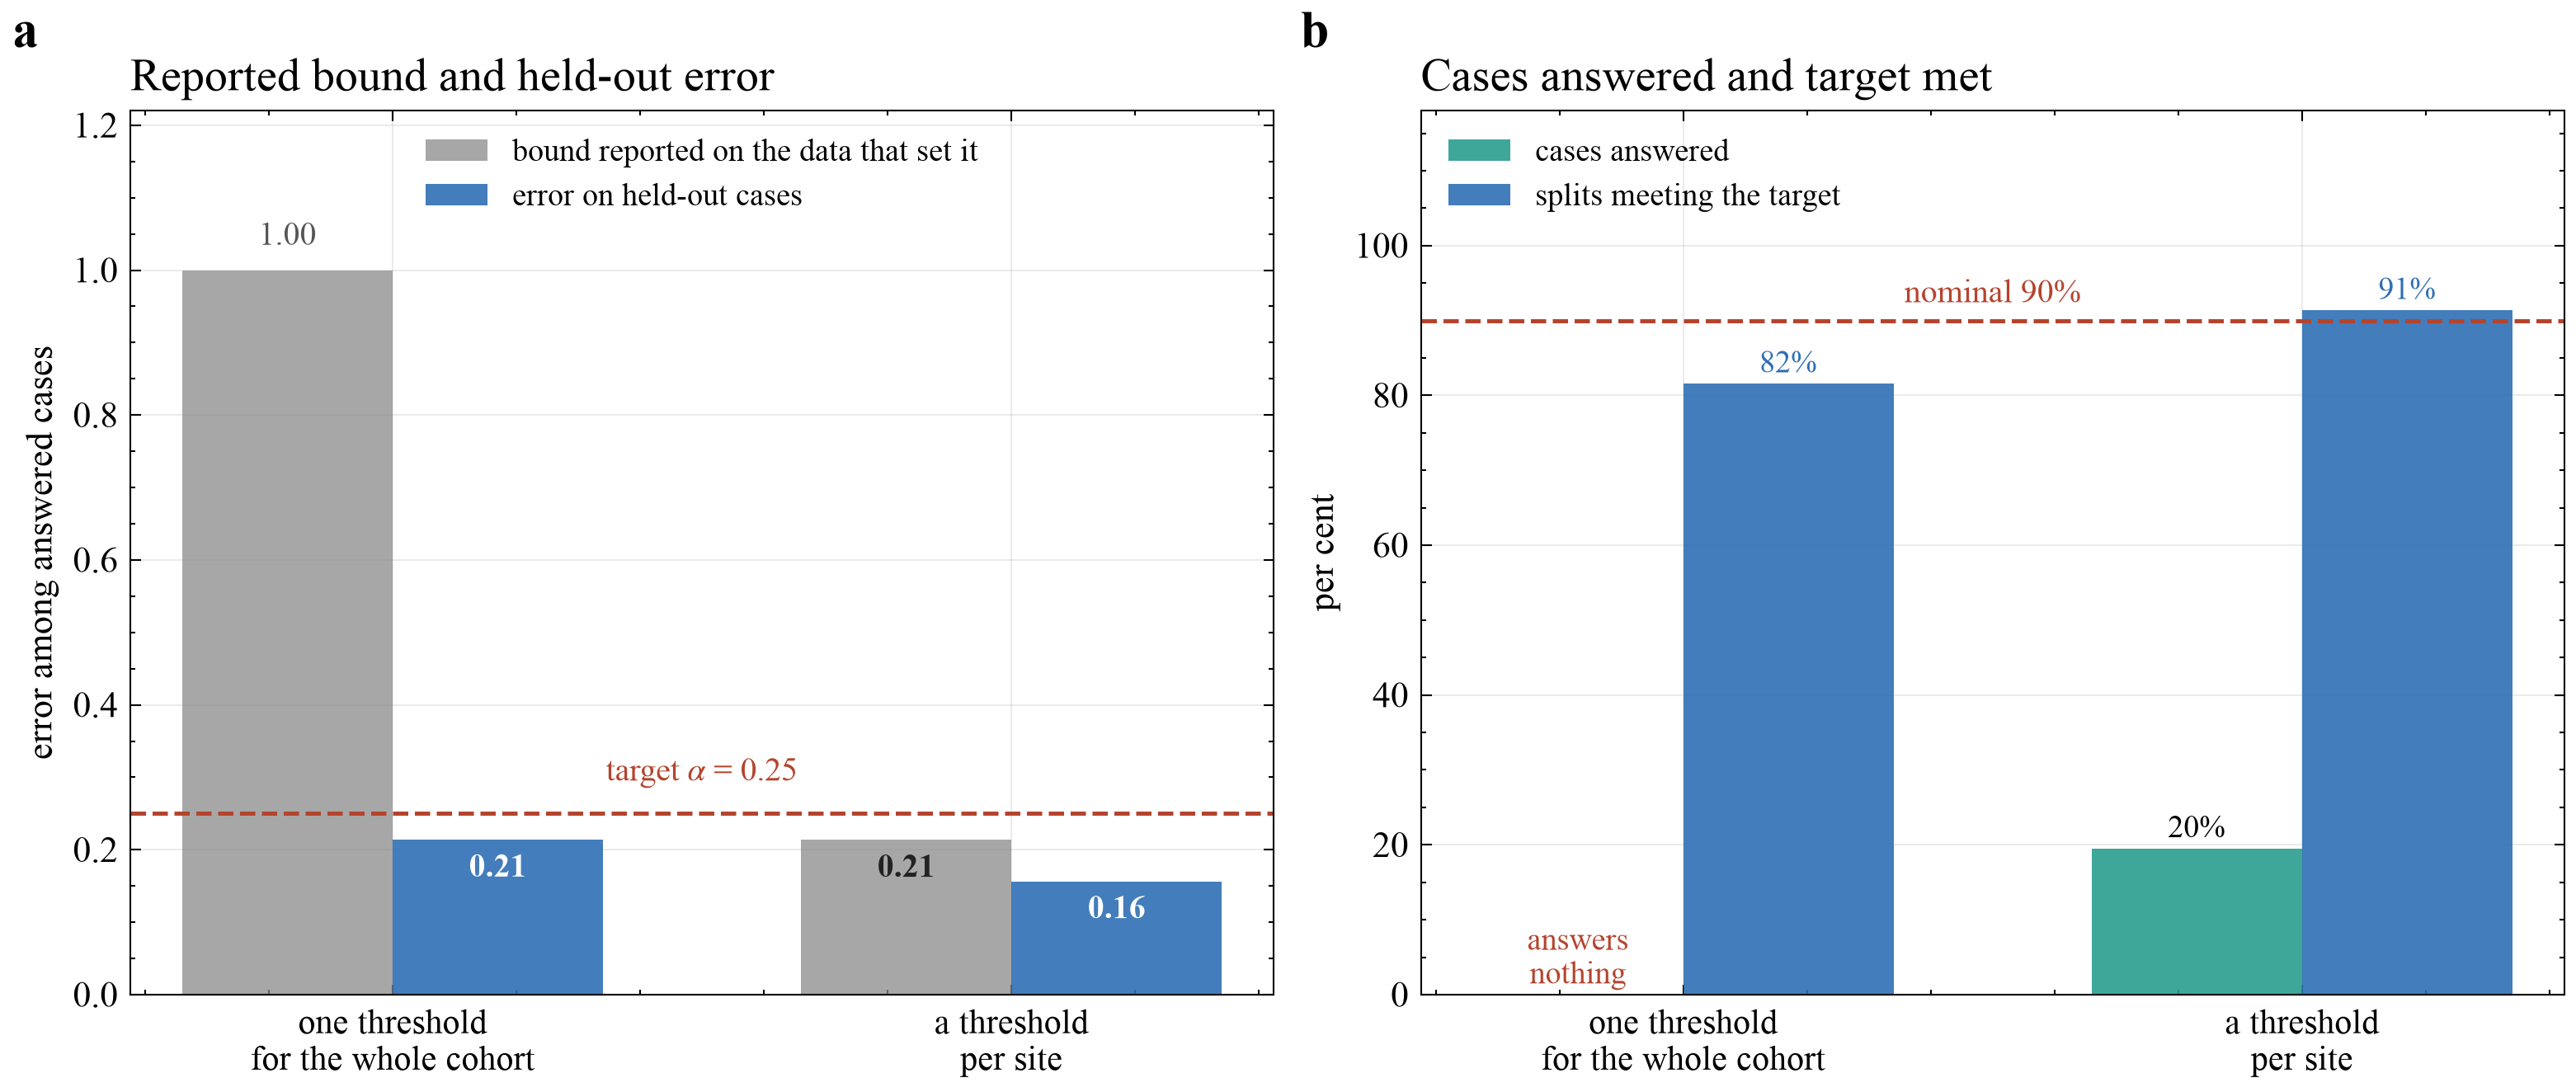
\includegraphics[width=\linewidth]{fig_guarantee}
\caption{The nominal error bound of the abstention rules under leave-one-site-out validation and its evaluation on held-out participants. (a) The error bound that each rule reports on the participants used to set it, against the error that the same rules incur on held-out cases. (b) The cost of each rule for obtaining that bound: the proportion of cases it answers, and the proportion of held-out splits in which it meets its target, against the nominal 90\%.}
\label{fig:abstention-guarantee}
\end{figure}

\section{Combining brain parcellations}
\label{sec:supp-atlas}

\subsection{Methods}
This secondary comparison examines whether connectivity described by more than one brain parcellation improves discrimination. In addition to the 200-region functional parcellation of Craddock et al. (CC200), the automated anatomical labelling atlas \citep{TzourioMazoyeretal2002} and the Harvard--Oxford probabilistic atlas are used, because these two atlases divide the brain on anatomical rather than functional grounds and therefore potentially carry complementary information. All three sets of regional time series are taken from the ABIDE Preprocessed Initiative \citep{Craddocketal2013,ABIDE_preprocessed_dataset}, using the C-PAC pipeline with band-pass filtering and without global-signal regression, so that the atlases differ in parcellation only and not in preprocessing. The Harvard--Oxford series are the distributed derivative \texttt{rois\_ho}, which holds 111 regions per participant, a count that is confirmed in every downloaded file. The derivative is based on the Harvard--Oxford cortical and subcortical structural atlases distributed with FSL, which cover 48 cortical and 21 subcortical structures segmented by the Harvard Center for Morphometric Analysis \citep{Makrisetal2006,Frazieretal2005,Desikanetal2006,Goldsteinetal2007}. Static tangent features are computed separately for each atlas, and the probabilities of the corresponding models are averaged for every combination of two and three atlases. The same outer folds, feature scaling, and classifier are used throughout, so that any difference in performance is attributable to the atlas information alone.

\subsection{Results}
Combining multiple atlases does not improve discrimination. CC200 alone gives a fold-mean AUROC of 0.756, compared with 0.749 when combined with the anatomical labelling atlas, 0.755 with the Harvard--Oxford atlas, and 0.752 with all three. The anatomical atlases perform lower on their own, at 0.692 and 0.717, indicating that the added atlases contribute little beyond CC200.

\section{Diagnostic-label uncertainty}
\label{sec:supp-label-noise}

\subsection{Methods}
Agreement between the Autism Diagnostic Interview--Revised (ADI-R) and the Autism Diagnostic Observation Schedule (ADOS) criteria is examined among autistic participants with complete scores for both instruments. The ADI-R criterion requires scores of at least 10 for social interaction, 8 for verbal communication, and 3 for restricted or repetitive behaviour \citep{Lordetal1994}, while the ADOS criterion requires a total score of at least 7. Agreement is summarised using the resulting $2\times2$ table, the discordance rate, and Cohen's $\kappa$. The ABIDE-I diagnostic label remains the classification outcome throughout. Concordance is then combined with Social Responsiveness Scale (SRS) data from non-autistic participants to explore the effect of possible label noise under the mutually contaminated model of \citet{Menonetal2015}. The autistic-label noise rate, $\varepsilon_1$, is initially set to half the observed disagreement rate $\eta$, while the non-autistic noise rate, $\varepsilon_0$, is estimated from the 137 non-autistic participants with available SRS totals as the proportion whose raw score is at least 60. With $\pi_1$ and $\pi_0$ denoting the proportions of autistic and non-autistic participants in the primary cohort, the corresponding accuracy ceiling is $1-(\pi_0\varepsilon_0+\pi_1\varepsilon_1)$. The observed AUROC and accuracy are also corrected using the same noise rates. Corrected AUROC is $(\mathrm{AUROC}-0.5)/(1-\varepsilon_0-\varepsilon_1)+0.5$, while corrected accuracy is $(\mathrm{accuracy}-(\varepsilon_0+\varepsilon_1)/2)/(1-\varepsilon_0-\varepsilon_1)$. The accuracy expression is exact for balanced accuracy but only approximate for accuracy because the diagnostic groups are unequal in size. These noise rates are not identifiable from the available data, because two instruments applied to one population do not uniquely determine sensitivity, specificity, and prevalence, and no participant is negative on both instruments. In addition, the conventional SRS threshold of 60 applies to a T-score, whereas the release provides raw totals. The accuracy ceiling and corrected performance are therefore reported as sensitivity ranges over $\varepsilon_1\in\{0,\eta/2,\eta\}$ and raw-total thresholds of 40, 50, 55, 60, and 70.

\subsection{Results}
Among 213 autistic participants with complete ADI-R and ADOS information, the instruments disagree in 15.0\% of cases: 13 meet criteria on the interview only, 19 on the observation only, and 181 on both, with none negative on both instruments. Under the assumptions of the Methods above, this corresponds to an illustrative attainable-accuracy range of approximately 0.85--0.99, as Figure~\ref{fig:label-ceiling} shows, while the observed accuracy of 0.707 remains about 0.14 below its lower bound. At the central noise rates defined above, the correction \citep{Menonetal2015} increases accuracy from 0.707 to 0.729 and AUROC from 0.776 to 0.806. Label uncertainty alone therefore does not account for the observed performance gap under these assumptions. However, the correction becomes larger under more pessimistic noise rates, and the data do not identify the true error rates. Cohen's $\kappa$ is slightly negative ($-0.078$), no participant is negative on both instruments, and the assumptions of the two-rater noise model are not fully supported. For these reasons, the analysis is treated as a sensitivity assessment rather than as a definitive estimate of the performance ceiling, and no point estimate of the ceiling is reported.

\begin{figure}[tbp]
\centering
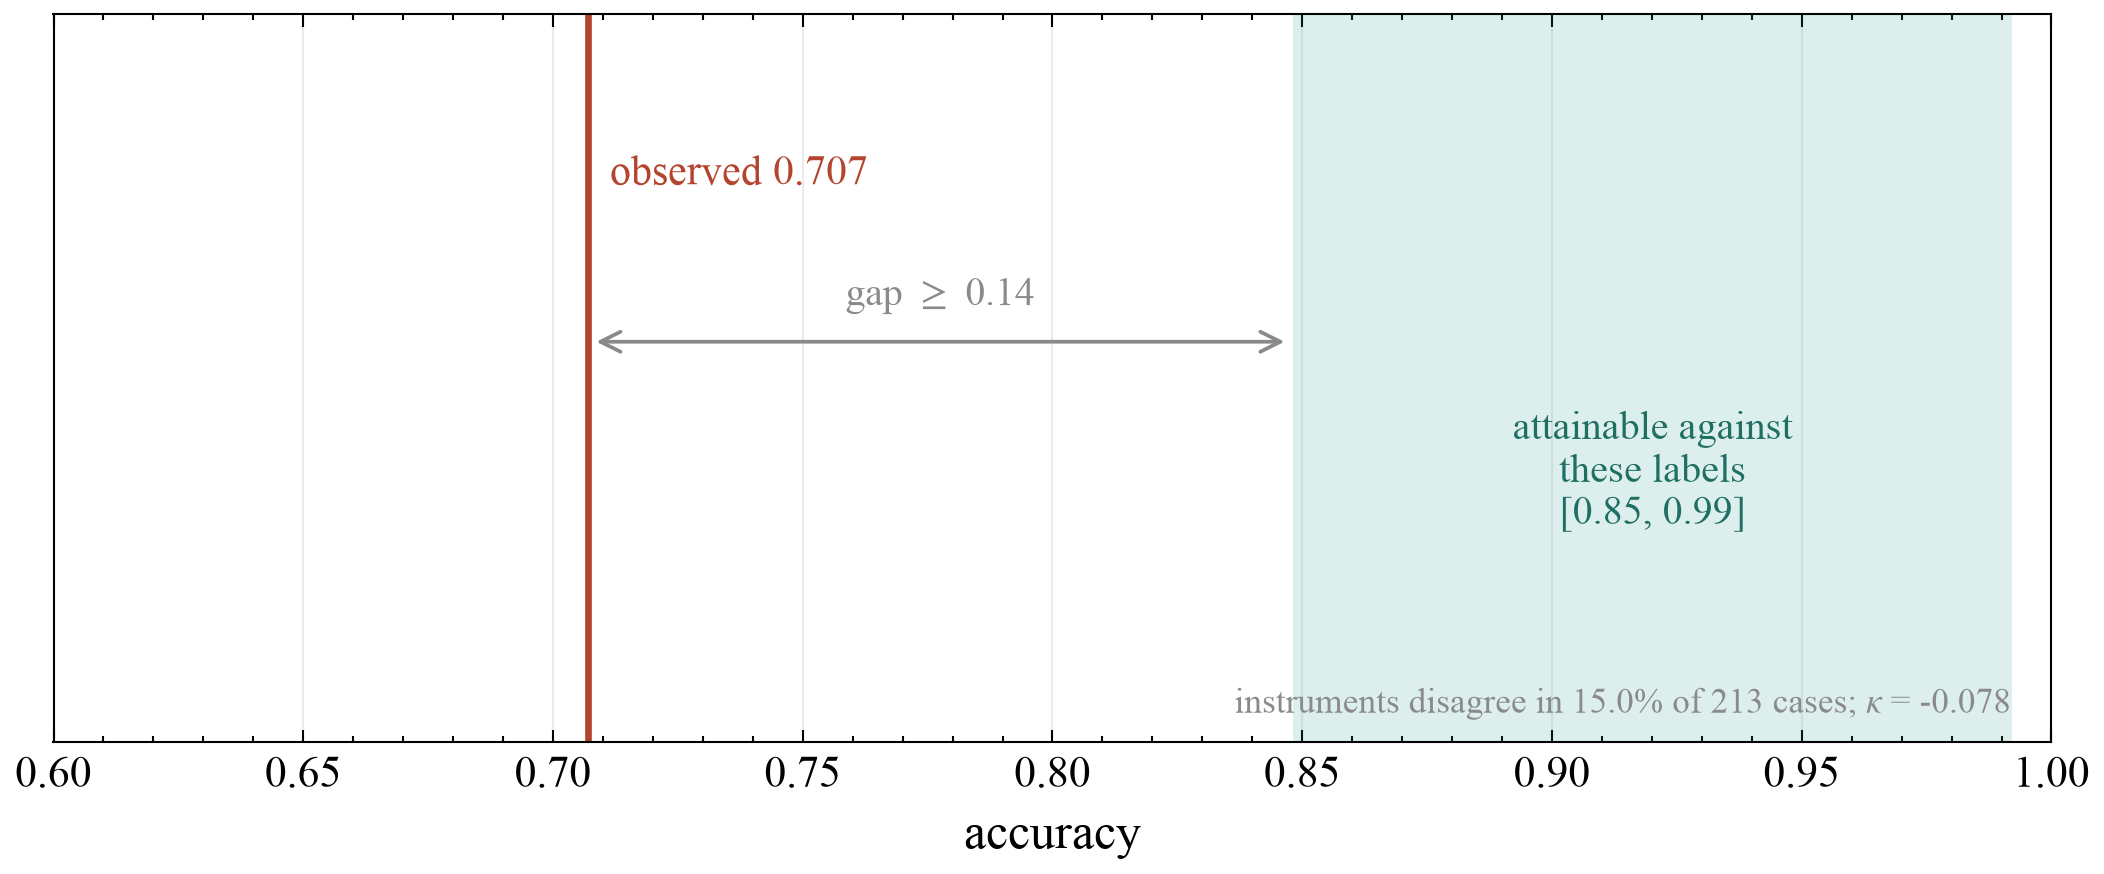
\includegraphics[width=0.9\linewidth]{fig_label_ceiling}
\caption{Observed accuracy against the range of accuracy attainable given the diagnostic labels under the assumptions of the label-noise sensitivity analysis. The range is illustrative and is not identified by the data.}
\label{fig:label-ceiling}
\end{figure}

\bibliographystyle{unsrtnat}
\bibliography{references}

\end{document}
